\documentclass[tikz, border=10pt]{standalone}
\usepackage{pgfplots}
\usepackage{amsmath}
\usetikzlibrary{backgrounds}
\pgfplotsset{compat=1.18}

\begin{document}
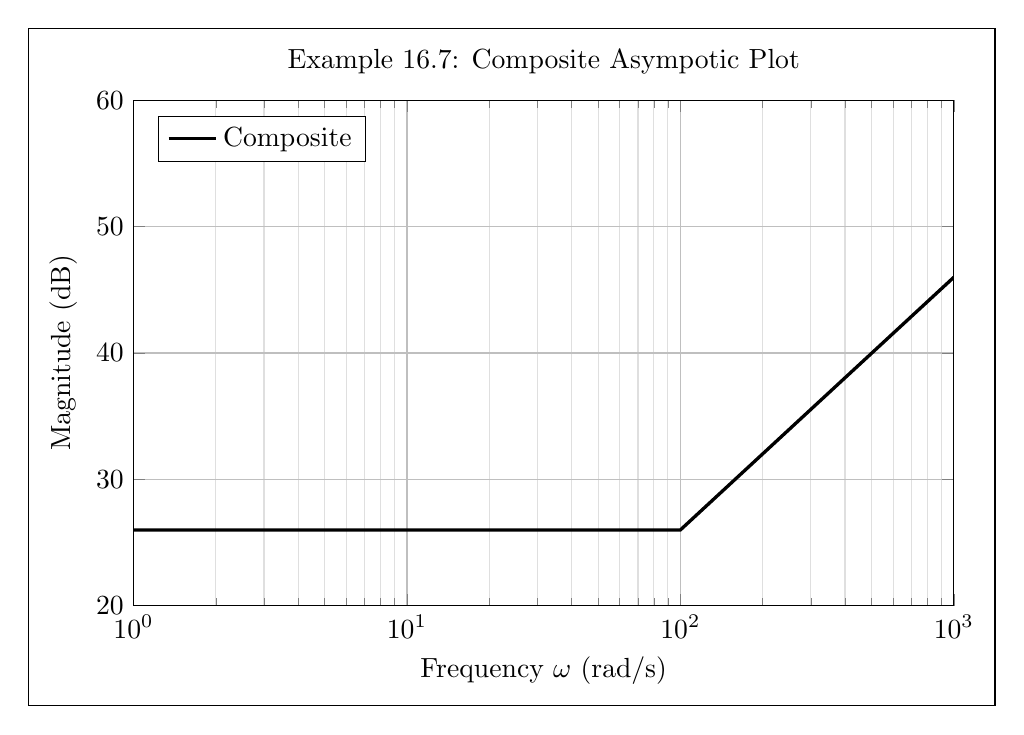
\begin{tikzpicture}[show background rectangle]
    \begin{semilogxaxis}[
        width=12cm, height=8cm,
        title={Example 16.7: Composite Asympotic Plot},
        xlabel={Frequency $\omega$ (rad/s)},
        ylabel={Magnitude (dB)},
        grid=both,
        xmin=1, xmax=1000,
        ymin=20, ymax=60,
        minor grid style={gray!25},
        major grid style={gray!50},
        legend pos=north west,
    ]

    % Composite: Sum of 26dB and Zero
    % <100: 26 + 0 = 26
    % >100: 26 + 20log(x/100)
    % At 1000, 26 + 20 = 46
    \addplot[black, very thick, domain=1:1000] coordinates {
        (1, 26) (100, 26) (1000, 46)
    };
    \addlegendentry{Composite}
    
    \end{semilogxaxis}
\end{tikzpicture}
\end{document}
